\chapter{Design and Implementation}

\section{Design}

The exact mechanisms of a lottery can be implemented in many ways. The following
describes the design choices made in this work.

The most important concept is that there is not only a single lottery contract
but rather one contract for each round of the lottery. One round consists of
players betting and the picking of a winner. After a winner has been chosen the
specific lottery is closed and a new lottery is deployed. The lotteries are
controlled via a central lottery factory that spawns new lotteries, knows of the
current active lottery, and is the interface by which the lottery issuer can
manage the lottery flow and the players can set there bets. The lottery factory
is also the owner of the bets made by players. The lottery instance themselves
do not have command over the bets. If there is no winner in a lottery round then
all bets made in that round are kept in the lottery factory and reused in the
next round. The issuer of the lottery factory cannot withdraw the balance
accumulated on the lottery factory.

The advantage of the separation of factory and lotteries is that each lottery
round is retrievable by its own address and the factory can be queried for the
list of all past lotteries. This seems more convenient than the case in which
only one lottery is reused for each round. We can avoid having to scan through
the blockchain to retrieve the transaction history of the lottery and
reconstruct its intermediary states.

Other design decisions are:
\begin{itemize}
  \item A player can bet multiple times on the same or different numbers in a
  single lottery round.
  \item The lottery issuer sets a ticket price which is the minimum price a player
  has to pay for his bet. The system does not prevent the player to pay more,
  but he does not get any benefits from it. 
  \item The issuer of the lottery factory sets the number range by providing a
  maximum number that can be bet.
\end{itemize}

The interactions of the lottery manager and the players with the lottery
systems are displayed Figure \ref{fig:use_case}. All interactions are happening
via the \texttt{LotteryFactory}. The lottery factory forwards the calls to the
current lottery. The users do not have to know or keep track of the concrete
lottery instances.

\begin{figure}[ht]
  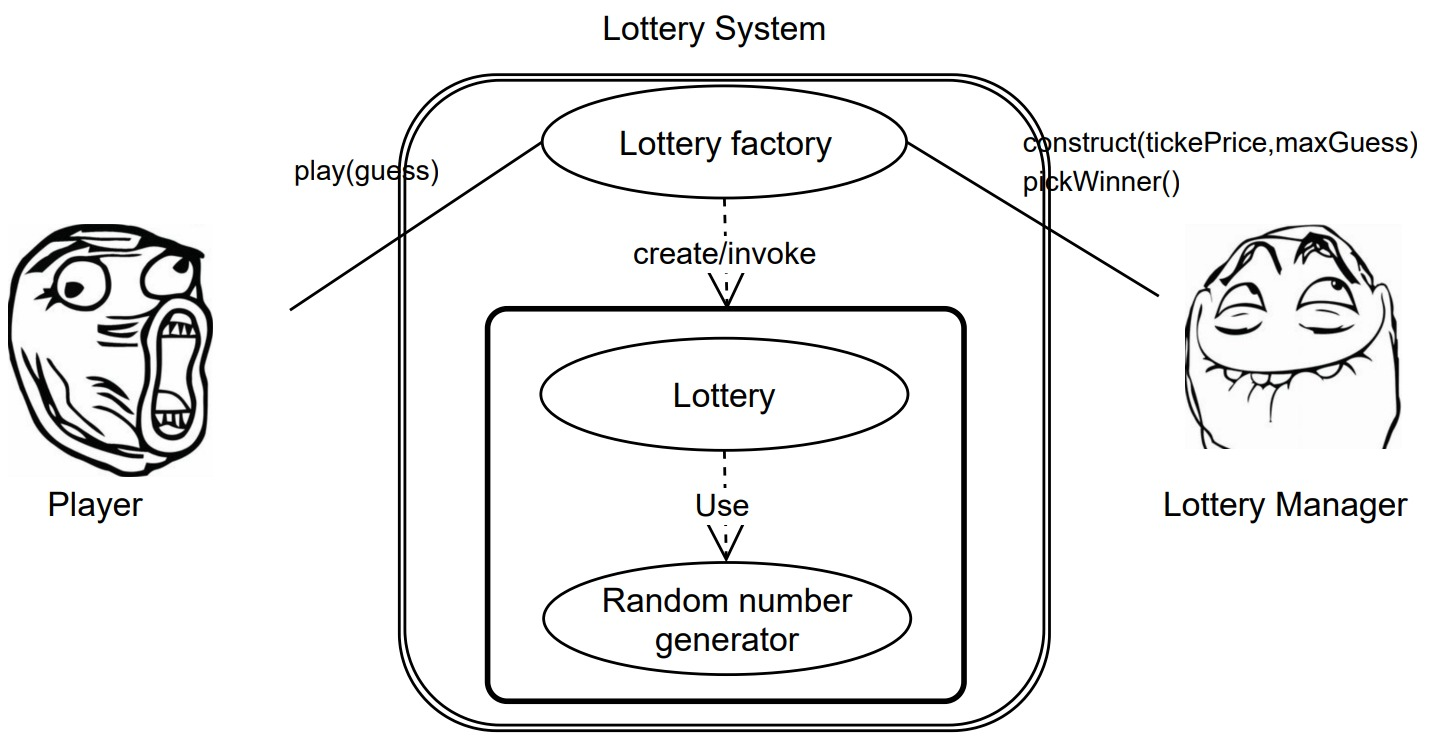
\includegraphics[width=\linewidth]{use_case.jpeg}
  \caption{Use case diagram of the lottery system.}
  \label{fig:use_case}
\end{figure}

In the following sections the details of the implementation are explained hand in hand
with the actual contract code. Figure \ref{fig:class_diagram} show the existing
classes/contracts which are part of the lottery system.

\begin{figure}[ht]
  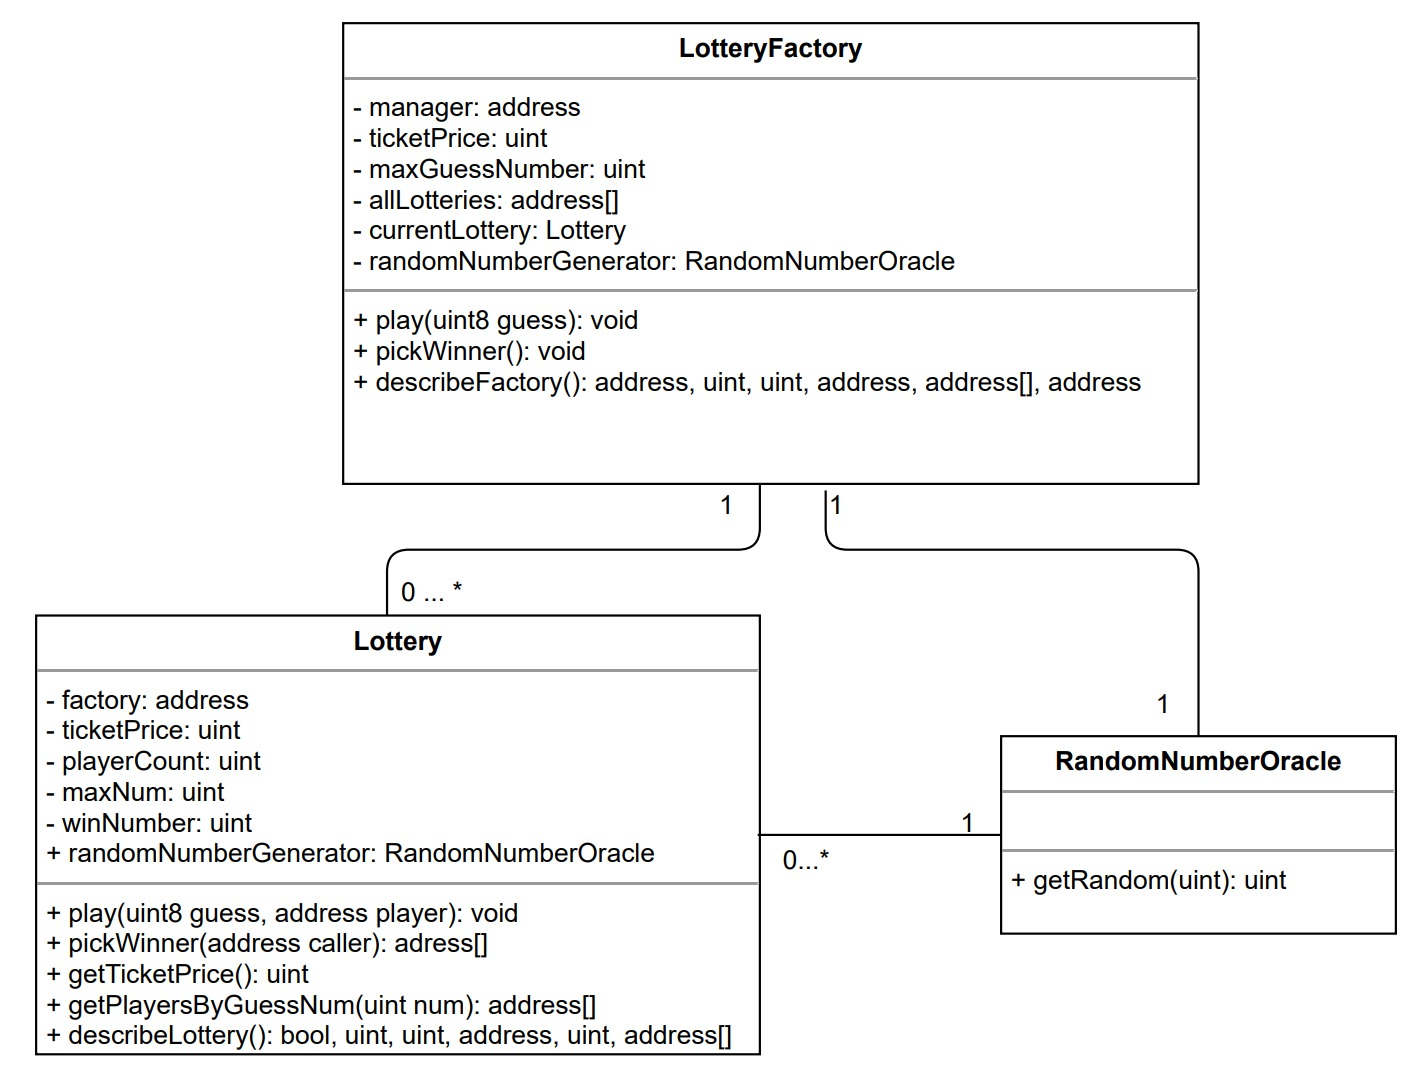
\includegraphics[width=\linewidth]{class_diagram.jpeg}
  \caption{Class diagram of the lottery system.}
  \label{fig:class_diagram}
\end{figure}


% ------------------------------------------------------------------------------

\section{Lottery Factory construction}

Once created, the \texttt{LotteryFactory} remembers the \texttt{manager} (the
address of the lottery issuer) for later checks. The ticket price and the
maximum guess number are chosen by the issuer, i.e. provided to the constructor,
and are fixed for all future lotteries. The lottery factory creates its own
\texttt{RandomNumberOracle} instance which will be called by all future lotteries
when a number has to be drawn. Finally, a first \texttt{Lottery} instance is
created which becomes the current lottery.

\begin{Verbatim}[fontsize=\tiny]
contract LotteryFactory {

    address manager;
    uint ticketPrice;
    uint maxGuessNumber;
    address[] allLotteries;
    Lottery currentLottery = Lottery(address(0x0));
    RandomNumberOracle randomNumberGenerator = RandomNumberOracle(address(0x0));

  constructor(uint _ticketPrice, uint _maxGuessNumber) public {
      manager = msg.sender;
      ticketPrice = _ticketPrice;
      maxGuessNumber = _maxGuessNumber;
      randomNumberGenerator = new RandomNumberOracle();
      currentLottery = new Lottery(_ticketPrice, address(this), 
          address(randomNumberGenerator), maxGuessNumber);
      allLotteries.push(address(currentLottery));
  }
\end{Verbatim}

% ------------------------------------------------------------------------------

\section{Playing the lottery}

For depositing a bet a player calls the \texttt{LotteryFactory.play()} method.
The \texttt{LotteryFactory} does basic checks for the validity of the bet and
calls the currently active \texttt{Lottery}'s \texttt{play()} method. The amount
of Ether sent with the bet are not transferred to the \texttt{Lottery} but are
kept in the \texttt{LotteryFactory}. The \texttt{Lottery} only keeps track of
the player address and his guess.

\begin{Verbatim}[fontsize=\tiny]
contract LotteryFactory {
  ...
  function play(uint8 guess) public payable {
      require(currentLottery != Lottery(address(0x0)), 
          "There is no lottery running.");
      require(msg.value >= currentLottery.getTicketPrice(), 
          "You have to send enough money.");
      currentLottery.play(guess, msg.sender);
  }
  ...
}

contract Lottery {
  ...
  function play(uint8 guess, address player) public {
      require(closed == false, "The lottery is closed.");
      require(guess <= maxNum, "Guess guess number not valid.");
      playersByNumber[guess].push(player);
      playerCount++;
  }
  ...
}
\end{Verbatim}

% ------------------------------------------------------------------------------

\section{Picking a winner}

The \texttt{LotteryFactory.pickWinner()} method can only be used by the
issuer/manager of the \texttt{LotteryFactory}. The \texttt{LotteryFactory}
forwards the call to the current \texttt{Lottery} which retrieves a random
number from the \texttt{RandomNumberOracle} and returns the players that have
bet on that number. The factory then distributes its current balance equally
between the winners. If there are no winners, the balance of the factory remains
untouched. The current \texttt{Lottery} is marked as closed and a new
\texttt{Lottery} is created which becomes the new current lottery.

\begin{Verbatim}[fontsize=\tiny]
contract LotteryFactory {
  ...
    function pickWinner() public {
        require(msg.sender == manager, "You are not authorized.");
        address[] memory winners = 
            currentLottery.pickWinner(address(this));
        if (winners.length != 0) {
            uint prize = address(this).balance / winners.length;
            for (uint i = 0; i < winners.length; i++) {
                winners[i].transfer(prize);
            }
        }
        currentLottery = new Lottery(ticketPrice, address(this), 
            address(randomNumberGenerator), maxGuessNumber);
        allLotteries.push(address(currentLottery));
    }
    ...
}

contract Lottery {
  ...
    function pickWinner(address caller) public returns (address[]) {
      require(caller == factory, 
          "You are not authorized to call this method.");
      require(closed == false, "The lottery is closed.");
      winNumber = randomNumberGenerator.getRandom(maxNum);
      closed = true;
      return (playersByNumber[winNumber]);
  ...
}

\end{Verbatim}
